\section{Project organisatie}

\subsection{Externe interfaces}
Het project is opgedragen door de VUB in het kader van de lessen "Software Engineering". De cliënten zijn Ragnhild Van Der Straeten \cite{rvdstrae} en assistent Jens Nicolay \cite{jnicolay}. De applicatie zal initieel op Wilma \cite{Wilma} staan, een multifunctionele Linux-server die wordt onderhouden door Dirk van Deun \cite{dvdeun}. \\

\subsection{Interne structuur}

\begin{figure}[h]
\centering
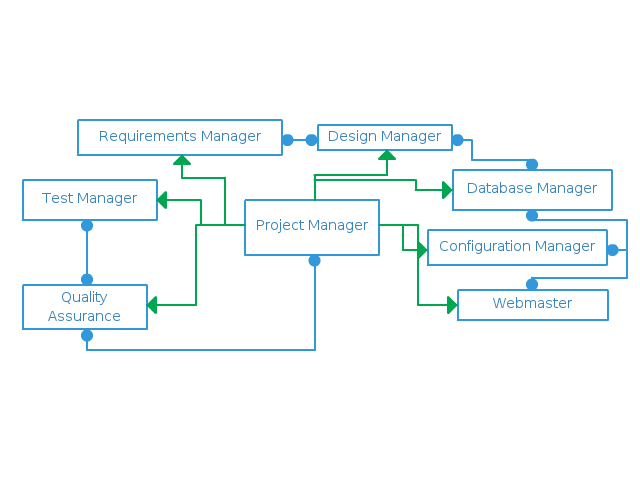
\includegraphics[width=\linewidth]{./Wiselib_intOrg.png}
\caption{Interne organisatie}
\label{fig:intorg}
\end{figure}

De groene pijlen duiden aan wie toezicht houdt over wie.\newline 
De blauwe pijlen duiden aan tussen wie er veel gecomuniceerd wordt.

\subsection{Rollen en verantwoordelijkheden}
De teamleden vullen verschillende rollen in.
De rollen en hun functies zijn: 

\begin{itemize}
\item Project Manager
\begin{itemize}
\item Leidt het team
\item Contactpersoon van het team
\item Bemiddelaar tijdens meningsverschillen
\item Verantwoordelijk voor de vergaderingen
\item Maakt SPMP en onderhoudt het
\end{itemize}

\item Configuration Manager
\begin{itemize}
\item Beheert de tools en libraries die gebruikt worden
\item Beheert GitHub
\item Maakt het SCMP en onderhoudt het
\end{itemize}

\item Database Manager
\begin{itemize}
\item Beheert de database
\item Maakt en onderhoudt het SDD samen met de Design Manager
\end{itemize}

\item Design Manager
\begin{itemize}
\item Maakt en onderhoudt het SDD 
\item Beslist en beheert het design van de toepassing en de database
\item Communiceert met de cliënt over het design
\end{itemize}

\item Test Manager
\begin{itemize}
\item Zorgt dat het programma aan voldoende testen wordt onderworpen
\item Documenteert en rapporteert de resultaten van de testen
\item Maakt een test database aan
\item Maakt en onderhoudt het STD
\end{itemize}

\item Quality Assurance
 \begin{itemize}
 \item Zorgt voor de kwaliteit van de code
 \item Is verantwoordelijk voor de kwaliteit van de applicatie
 \item Zorgt ervoor dat aan alle nodige requirements voldaan zijn
 \item Maakt en onderhoudt het SQAP
 \end{itemize}
 
\item Requirements Manager
\begin{itemize}
\item Maakt en onderhoudt het SRS
\item Beslist de prioriteiten van de requirements
\item Communiceert met de cliënt over de requirements
\end{itemize}

\item Webmaster 
\begin{itemize}
\item Maakt en onderhoudt de website
\end{itemize}
\end{itemize}
 \newpage

